\chapter{\textbf{Methodik}}
\label{chap:methods}

Nach der Einordnung des Stands der Technik wird in diesem Kapitel die im Rahmen der Arbeit angewandte Methodik systematisch dargestellt. 
Zunächst wird die Entwicklung der Anwendung auf Basis des Spiralmodelles (vgl. Kap. \ref{sec:spiral-model}) beschrieben und der technische Aufbau des lauffähigen Prototypen erläutert.
Darauf aufbauend werden die Durchführung der Interviews sowie die Entwicklung und Bearbeitung der Aufgabenstellungen dargestellt; anschließend erfolgt die Validierung der erzeugten \gls{llm}-Ausgaben.
Den Abschluss bildet die strukturierte Aufbereitung der erhobenen Daten als Grundlage für die spätere Auswertung.

\section{KI-Anwendung für Interviews}
\label{sec:app}

Zur Evaluierung der Fähigkeiten von künstlicher Intelligenz in digitalen Planungsprojekten wurde im Rahmen dieser Bachelorarbeit eine Anwendung entwickelt, die im Rahmen der Interviews eingesetzt werden konnte.
Die Anwendung wurde bewusst als methodisches Werkzeug konzipiert, um die Interaktion der Probanden mit dem \gls{llm} unter vergleichbaren Rahmenbedingungen zu ermöglichen.
Damit konnte eine nachvollziehbare Grundlage geschaffen werden, auf deren Basis die Qualität der erzeugten Antworten systematisch betrachtet werden kann.
Während der Entwicklungsfokus auf der genannten Kernfunktion lag, wurden Benutzererfahrung und zusätzliche Funktionen nur sekundär betrachtet und flossen lediglich teilweise in Entwicklungsentscheidungen ein. 
Ein wichtiger Teil des Konzeptes war die Möglichkeit mehrere \gls{ifc}-Modelle gleichzeitig zu laden, um dem in der Praxis angewandten Aufteilen von Modellen nach Fachdisziplin (vgl. Kap. \ref{sec:open-closed-bim}) gerecht zu werden. \\

Die Struktur der Entwicklung orientierte sich am Spiral-Modell (vgl. Kap. \ref{sec:spiral-model}). Zunächst wurde ein Konzept erarbeitet, das die grundlegenden Anforderungen und Ziele der Anwendung festlegte.
Darauf folgte eine Vorentwicklung, in der die technologische Machbarkeit überprüft wurde und anschließend in der Entwicklung des ersten Prototypen mündete.
Die letzte Phase stellte die Entwicklung des lauffähigen Prototypen dar, welcher für die Interviews eingesetzt wurde.
Eine vollständige Implementierung für ein Release war im Rahmen der Bachelorarbeit jedoch nicht vorgesehen, da dies die zur Verfügung stehenden Ressourcen überschritten hätte. \\

Im folgenden Abschnitt wird näher auf das erarbeitete Konzept der entwickelten Anwendung eingegangen.

\subsection{Konzept}
\label{sec:app-concept}

Als Kern der Anwendung wurde eine textbasierte Eingabe vorgesehen, über die Probanden direkt mit dem \gls{llm} kommunizieren können.
Die gewählte Form der Interaktion reduziert technische Hürden und unterstützt damit eine möglichst direkte Bearbeitung der Aufgabenstellungen.
Darüber hinaus war eine einfache Konfiguration der Variablen, die das \gls{llm} beeinflussen, für eine schnelle Entwicklung und schrittweise Verbesserung der Anwendung erforderlich.
Dies umfasst neben dem Systemprompt auch die dem \gls{llm} zur Verfügung gestellten Werkzeuge (tool calling) sowie zusätzlich eingebundenes Wissen.
Auf diese Weise konnte die inhaltliche Steuerung des Modells gezielt angepasst werden, ohne die grundlegende Systemarchitektur während der Entwicklung ändern zu müssen. \\

Bei der Anbindung des \gls{llm} wurde auf externe Dienstleister zur Bereitstellung der \gls{llm}-Funktionalität gesetzt, 
um den Betrieb der entsprechenden \gls{llm} aus der Bachelorarbeit auszulagern und den Entwicklungsaufwand zu reduzieren.
Alle eingesetzten \gls{llm} besitzen ein \gls{api}, das mit dem OpenAI \gls{api}-Standard kompatibel ist.
Dies ermöglicht einen Tausch des verwendeten \gls{llm}, ohne die Anwendung grundlegend bearbeiten zu müssen.
Damit wurde zugleich sichergestellt, dass Modellwechsel oder Anpassungen an der Modellwahl den methodischen Ablauf der Interviews nicht beeinflussen. \\

Der Nutzer übermittelte bei der Bedienung Fragen über die Anwendung an das \gls{llm}, das auf Basis des Systemprompts und des im \gls{ifc}-Modell vorhandenen Wissens eine Antwort ausgibt.
Damit wurde ein klarer und einheitlicher Ablauf geschaffen, der die Bearbeitung der Aufgaben sowie die spätere Auswertung der Antworten unterstützt. \\

\subsection{Vorentwicklung und technische Machbarkeit}
\label{sec:app-iteration-1}

Um zu überprüfen, ob die im Konzept geplanten Technologien in Kombination zu einer funktionsfähigen Anwendung führen, 
wurde am Anfang des Entwicklungsprozesses die technische Machbarkeit mit einer Vorentwicklung evaluiert.
Dabei basierte die Vorentwicklung auf einem vorgefertigten \gls{mcp}-Server, der in Python mit der FastMCP-Bibliothek umgesetzt wurde \cite{github2025bonsaimcp}.
Als technische Grundlage wurde die öffentlich verfügbare 3D-Bearbeitungssoftware Blender verwendet, um \gls{ifc}-Modelle zu laden und zu bearbeiten.
Da der \gls{ifc}-Standard in Blender nicht nativ verfügbar ist, wurde die Erweiterung Bonsai eingesetzt, die von IfcOpenShell bereitgestellt wird \cite{bonsai2026blenderextensions}. \\

\begin{table}[!htb]
    \centering
    \caption[Bereitgestellte Werkzeuge vom vorgefertigten \gls{mcp}-Server]{Alle Werkzeuge, welche der vorgefertigte \gls{mcp}-Server bereitgestellt hat.}
    \label{tab:iteration1tools}
    \begin{tabular}{L{6cm} L{8cm}}
        \hline
        \textbf{Name} & \textbf{Beschreibung} \\
        \hline

        \texttt{get\_ifc\_project\_info} & Gibt grundsätzliche Projektinformationen über das \gls{ifc}-Modell zurück. Neben Metadaten, wie Name und Beschreibung umfasst dies die Anzahl aller verfügbaren \gls{ifc}-Entitäten. \\

        \texttt{list\_ifc\_entities} & Durchsucht das \gls{ifc}-Modell auf Basis gegebener Suchparameter nach \gls{ifc}-Entitäten. Als Suchparameter stehen der \gls{ifc}-Entitätstyp und die Möglichkeit zur Begrenzung der Ergebnisanzahl zur Verfügung.  \\

        \texttt{get\_ifc\_properties} & Gibt alle Eigenschaften eines einzelnen Bauteils im geladenen \gls{ifc}-Modell auf Basis der globalen Identifikation oder der Nutzerselektion in Blender zurück. \\

        \texttt{get\_ifc\_spatial\_structure} & Gibt den strukturellen Aufbau des \gls{ifc}-Modells zurück. Dabei wird die Beziehung von Grundstücken (IfcSite), Gebäuden (IfcBuilding), Geschossen (IfcBuildingStorey) und einzelnen Räumen bzw. Flächen (IfcSpace) dargestellt. \\

        \texttt{get\_ifc\_relationships} & Gibt alle Beziehungen eines einzelnen Bauteils im geladenen \gls{ifc}-Modell auf Basis der globalen Identifikation oder der Nutzerselektion in Blender zurück. \\

        \texttt{get\_selected\_ifc\_entities} & Gibt grundsätzliche Informationen über die vom Nutzer in Blender selektierten Bauteile zurück. \\

        \texttt{export\_ifc\_data} & Erstellt eine als \gls{json} strukturierte oder als Tabelle formatierte Datei, welche die Struktur des \gls{ifc}-Modells abbildet. \\

        \texttt{place\_ifc\_object} & Platziert eine gewählte \gls{ifc}-Entität an der angegebenen Position. Dabei können Koordinaten und Rotation angepasst werden. \\

        \texttt{get\_ifc\_quantities} & Gibt Mengenwerte von \gls{ifc}-Entitäten zurück. \\

        \texttt{get\_ifc\_total\_structure} & Als Erweiterung von \texttt{get\_ifc\_spatial\_structure} werden zusätzlich die darunterliegenden \gls{ifc}-Entitäten ausgegeben, die einen Bezug zu einem einzelnen Raum bzw. einer Fläche (IfcSpace) besitzen. \\
        
        \hline
    \end{tabular}
\end{table} 

Um dem \gls{llm} den Zugriff auf Modellinhalte und Bearbeitungsfunktionen zu ermöglichen, wurde eine zusätzliche Erweiterung genutzt, die gemeinsam mit dem \gls{mcp}-Server bereitgestellt wurde.
Die Kommunikation zwischen Server und Blender erfolgte über eine Socket-Verbindung.
Dabei wurden Werkzeugaufrufe einschließlich ihrer Parameter vom \gls{mcp}-Server an die in Blender installierte Erweiterung übermittelt, die die Befehle an Bonsai weiterleitete.
Der \gls{mcp}-Server übernahm damit die Rolle einer Schnittstelle zwischen \gls{llm} und Modellbearbeitung \cite{github2025bonsaimcp}.
In Tabelle \ref{tab:iteration1tools} sind die durch den \gls{mcp}-Server bereitgestellten Werkzeuge gelistet. \\

Im folgenden Abschnitt wird die Entwicklung des Prototyps erläutert, welcher auf Basis der Vorentwicklung entwickelt wurde.

\subsection{Entwicklung des Prototypen}
\label{sec:app-iteration-2}

Auf Basis der im vorherigen Kapitel vorgestellten Vorentwicklung wurde im Rahmen der Prototypenentwicklung ein selbst entwickelter \gls{mcp}-Server geschaffen. 
Dieser wurde in der Programmiersprache Python unter Verwendung der FastMCP-Bibliothek umgesetzt \cite{gofastmcp2026welcome}.
Im Unterschied zur Vorentwicklung lag der Schwerpunkt auf einer gezielten Reduktion der bereitgestellten Werkzeuge. 
Statt einer breiten Abdeckung von Modellbearbeitungsfunktionen wurden nur noch Werkzeuge zur Wissensgewinnung bereitgestellt. \\

Die bereitgestellten Werkzeuge entsprechen in ihrer Funktion weitgehend der Vorentwicklung, verwenden jedoch als \gls{ifc}-Bibliothek IfcOpenShell anstelle der Kombination aus Bonsai und Blender als \gls{ifc}-Viewer. 
Dies ermöglicht die eigenständige Definition der Extraktionslogik aus den geladenen Modellen. Im Hinblick auf die Leistungsfähigkeit des \gls{llm} erlaubt dies eine genauere Kontrolle über den bereitgestellten Kontext \cite{ifcopenshell_github}. \\

Für die textbasierte Interaktion mit dem \gls{llm} wurde Open WebUI als Oberfläche genutzt.
Die Software ermöglichte die Anbindung an unterschiedliche \gls{llm} sowie die Einbindung eigener \gls{mcp}-Server.
Zusätzlich bot sie eine praktikable Grundlage für den Export von Nachrichtenverläufen und damit für die spätere Analyse der im Interview erzeugten Kommunikation \cite{openwebui2026home}. \\

Nach der Definition des Prototypen wird im folgenden Abschnitt die Entwicklung des lauffähigen Prototypen (operational prototype) erläutert.

\subsection{Entwicklung des lauffähigen Prototypen}
\label{sec:app-final-iteration}

Der im vorherigen Abschnitt definierte Prototyp diente zusammen mit dem Konzept als Grundlage für die Entwicklung des lauffähigen Prototypen (operational prototype).
Im Mittelpunkt der Entwicklung stand dabei die Anbindung eines externen Datensatzes als Datenquelle, die eine effizientere Bereitstellung von Wissen für das \gls{llm} ermöglicht.
Die Struktur des Datensatzes ist in Tabelle \ref{tab:103_app-data-structure} dargestellt und umfasst Informationen zu Bauteilen, Systemen, Materialien und Geschossen, die in den bereitgestellten \gls{ifc}-Modellen enthalten sind.
Dabei entspricht jede Zeile einem einzelnen Eigenschaftswert, einer Systembeschreibung oder anderen einzelnen Informationseinheit, die mit einem Bauteil oder einem anderen Element im Modell verknüpft ist. \\
\begin{table}[!htb]
    \centering
    \caption{Struktur des externen Datensatzes für den lauffähigen Prototypen}
    \label{tab:103_app-data-structure}
    \begin{tabular}{C{3cm} C{1.5cm} L{6.5cm}}
        \hline
        \textbf{Spalte} & \textbf{Typ} & \textbf{Beschreibung} \\
        \hline

        element\_uuid & text & Identifikation jedes Bauteils \\

        model\_id & text & Referenz zum Modell \\

        element\_type & text & IFC-Entitätstyp \\

        property\_id & text & Identifikation der Eigenschaft \\

        property\_name & text & Name der Eigenschaft \\

        property\_value & text & Wert der Eigenschaft \\

        property\_description & text & Beschreibung der Eigenschaft \\

        property\_type & text & Typklassifikation der Eigenschaft \\

        property\_valuetype & text & Datentyp des Wertes \\

        pset\_name & text & Name des Property Sets  \\

        pset\_type & text & Typ des Property Sets \\

        pset\_description & text & Beschreibung des Property Sets \\

        system\_uuid & text & Identifikation des Systems \\

        system\_name & text & Name des Systems \\

        system\_type & text & Typ des Systems \\

        system\_description & text & Beschreibung des Systems \\

        material\_name & text & Name des Materials \\

        material\_category & text & Kategorie des Materials \\

        material\_description & text & Beschreibung des Materials \\

        material\_thickness & text & Dicke des Materials \\

        storey\_uuid & text & Identifikation des Geschosses \\

        storey\_name & text & Name des Geschosses \\

        storey\_longname & text & Vollständiger Name des Geschosses \\

        \hline
    \end{tabular}
\end{table}


Zur Integration des Datensatzes wurde eine vollständige Web-Anwendung geschaffen (full stack web application), die die methodische Kontrolle des gesamten Ablaufs der Anfrageverarbeitung ermöglichte.
Des Weiteren war die genaue Definition des Systemprompts sowie die Strukturierung der Anfragearchitektur ein wesentliches Mittel, um die Qualität der \gls{llm}-Abfragen zu steigern.
Für die Entwicklung der Web-Anwendung wurde TypeScript als Programmiersprache eingesetzt, um die Kommunikation zwischen Frontend und Backend zu vereinfachen. \\

Der lauffähige Prototyp wurde im Rahmen der Interviews mit den Probanden eingesetzt, die im nachfolgenden Abschnitt näher beschrieben werden.

\section{Interviews}
\label{sec:interviews}

Um die entwickelte \gls{llm}-Anwendung mit Probanden zu testen, wurden Interviews durchgeführt. Dabei handelte es sich um Einzelinterviews, die in Form einer Videokonferenz durchgeführt wurden.
Dies reduzierte die Nutzung von Ressourcen für die Koordination der Interviewtermine erheblich, da die Verfügbarkeit von Probanden durch das ortsunabhängige Format verbessert wurde.

Zur inhaltlichen Nachvollziehbarkeit wurde während der Gespräche ein grobes Gedankenprotokoll erstellt. Dieses diente als ergänzende Grundlage für die spätere Analyse der vom \gls{llm} erzeugten Ausgaben und half dabei, zentrale Beobachtungen aus der Interaktion systematisch festzuhalten.
Der Ablauf der Interviews ist in den folgenden Unterkapiteln schrittweise dargestellt, um die einzelnen methodischen Schritte transparent zu machen.

\subsection{Zuordnung zur Probanden-Gruppe}

Im ersten Schritt des Interviews wurde jeder Proband einer der beiden definierten Probanden-Gruppen zugewiesen. Dies erfolgte auf Basis der in Tabelle \ref{tab:103_interview-core-questions} gezeigten Fragen.

\begin{table}[!htb]
    \centering
    \caption{Den Probanden gestellte Fragen zur Zuordnung zu den Probanden-Gruppen}
    \label{tab:103_interview-core-questions}
    \begin{tabular}{C{2cm} L{11cm}}
        \hline
        \textbf{Index} & \textbf{Frage}\\
        \hline

        1 & Seit wie vielen Jahren haben Sie Ihre aktuelle Jobposition inne? \\

        2 & Wie viel Prozent der wöchentlichen Arbeitszeit beschäftigen Sie sich mit digitaler datengetriebener Planung? \\

        3 & Wie viel \% der wöchentlichen Arbeitszeit beschäftigen Sie sich mit der Koordination von Projekten oder Teammitgliedern? \\

        \hline
    \end{tabular}
\end{table}

Für die Zuordnung wurde Frage 2 als zentrales Kriterium gewichtet, da sie den unmittelbaren Anteil aktiver Tätigkeiten in der digitalen datengetriebenen Planung abbildet. 
Ergänzend wurden Frage 1 und Frage 3 herangezogen, um Probanden differenziert einzuordnen, die zwar einen geringeren operativen Anteil in diesem Aufgabenfeld aufweisen, 
jedoch aufgrund ihrer Berufserfahrung sowie ihrer fachlichen und organisatorischen Verantwortung weiterhin der Probanden-Gruppe A zugeordnet werden konnten. \\

Nach der Zuordnung der Probanden zu den entsprechenden Gruppen folgt in den nächsten beiden Unterkapiteln die Darstellung des zweiten Interviewschritts: 
zunächst die Entwicklung von Aufgabenstellungen durch Probanden-Gruppe A und anschließend die Bearbeitung dieser Aufgabenstellungen durch Probanden-Gruppe B.

\subsection{Entwicklung von Aufgabenstellungen durch Probanden-Gruppe A}
\label{sec:aufgabenstellung-gruppe-a}

Der zweite Schritt der Interviews für die Probanden-Gruppe A bestand aus der Entwicklung von Aufgabenstellungen. 
Dabei wurde die folgende Leitfrage entwickelt, um den Probanden einen Einstieg in das Interview zu ermöglichen: \\

\say{Ihnen steht eine unangelernte Hilfskraft zur Verfügung, für die Sie eine Aufgabe für ein exemplarisches digitales Modell formulieren sollen. Welche Aufgaben fallen Ihnen dazu in Stichworten ein?} \\

Zusätzlich zur genannten Leitfrage wurde den Probanden der Gruppe A der Rahmen für die Aufgabenstellungen erläutert. 
Es wurde dabei auf Aufgabenstellungen abgezielt, welche eine einzige Problemstellung betreffen. 
Besondere Priorität hatte dabei die Identifizierbarkeit des Kernproblems der Aufgabenstellung.
Für Probanden der Gruppe B sollte dabei erkenntlich sein, welches Ziel sie zu erreichen hatten. 
Dies schloss die Verwendung von Fachbegriffen nicht aus, da Probanden das \gls{llm} als Hilfsmittel einsetzen konnten.
Jedoch wurde explizit auf eine Kombination aus mehreren Aufgaben in einer einzelnen Aufgabenstellung verzichtet, 
um den Fokus der Probanden pro Aufgabenstellung auf ein einzelnes zu lösendes Problem zu lenken.

\subsection{Durchführung der Aufgabenstellung durch Probanden-Gruppe B}
\label{sec:aufgabenstellung-gruppe-b}
Im Vergleich zur Probanden-Gruppe A bestand der zweite Schritt des Interviews für die Probanden-Gruppe B aus der Bearbeitung der im vorherigen Unterkapitel (vgl. Kap. \ref{sec:aufgabenstellung-gruppe-a}) genannten Aufgabenstellungen. \\

Zu Beginn erhielten die Probanden eine kurze Einführung in Zielsetzung und Ablauf des Interviews. Die Einführung erfolgte bewusst ohne die Vorgabe eines starren Schemas und ohne inhaltliche Vorwegnahme möglicher Lösungswege. 
Zusätzlich wurde das Interviewdatum erfasst, um die spätere Extraktion der zugehörigen Nachrichten aus der Datenbank eindeutig zuordnen zu können. \\

Anschließend wurden die einzelnen Aufgabenstellungen nacheinander präsentiert und in festgelegter Reihenfolge bearbeitet. 
Dabei wurden keine zusätzlichen fachlichen Hinweise gegeben, sodass die Aufgabenbearbeitung ausschließlich auf der jeweiligen Aufgabenbeschreibung und der Interaktion mit dem \gls{llm} beruhte. \\

Die Probanden formulierten ihre Eingaben selbstständig und übermittelten diese aus technischen Gründen an den Interviewführer, der die Eingaben mithilfe der bereitgestellten Anwendung an das \gls{llm} weitergab. 
Sämtliche Eingaben sowie die jeweils erzeugten Antworten wurden fortlaufend in einem Gedankenprotokoll dokumentiert, um den Bearbeitungsverlauf später nachvollziehbar auswerten zu können. \\

Eine Aufgabenstellung galt als abgeschlossen, sobald der Proband das angestrebte Ziel als erreicht bewertete. 
Falls die erzeugten Ergebnisse deutlich von der Aufgabenstellung abwichen und keine zielführende Weiterbearbeitung erkennbar war, wurde die Bearbeitung dieser Aufgabe abgebrochen. 
Sofern im Verlauf der Bearbeitung Exportdateien, beispielsweise im CSV-Format, erzeugt wurden, wurden diese für die weitere Analyse lokal gespeichert. \\

Die \gls{llm}-Ausgaben, Dateierzeugnisse und andere Daten wurden danach auf Basis der im folgenden Abschnitt definierten Methodik validiert.

\section{Validierung der \gls{llm}-Ausgabe}
\label{sec:datenvalidierung}

Bevor die im Rahmen der Interviews gewonnenen Daten aufbereitet und ausgewertet werden konnten, wurden alle \gls{llm}-Ausgaben auf Richtigkeit geprüft. \\

Für die Überprüfung von Attributen und Struktur des digitalen Modells wurde ein Modellviewer eingesetzt, der mit dem \gls{ifc}-Standard kompatibel ist.
Es handelte sich dabei um BIMcollab Zoom, eine von BIMcollab entwickelte Software für die Prüfung und Qualitätsanalyse von digitalen datengetriebenen Gebäudemodellen.
BIMcollab Zoom unterstützt allgemein die Prüfung auf Kollisionen von Elementen, die Qualitätssicherung der verknüpften Parameter sowie die Durchsetzung von Standards für jedes Projekt \cite{bimcollabUnknownZoom}. \\

Zusätzlich bietet BIMcollab Zoom die Möglichkeit, bestehende Modelldaten auf Basis definierter Regeln zu restrukturieren sowie beliebige Parameter und Elemente farblich zu visualisieren.
Die Integration in andere Produkte von BIMcollab, wie BIMcollab Twin, eine \gls{cde}, oder BIMcollab Nexus, eine Kommunikationsplattform für Issues, ist ein wichtiger Teil von BIMcollab Zoom \cite{bimcollabUnknownZoom}. \\

Im Rahmen der Bachelorarbeit wurden damit unter anderem einzelne Elemente, beispielsweise technische Geräte, die vom \gls{llm} direkt erwähnt wurden, durch Selektion in BIMcollab Zoom geprüft.
Dabei wurden alle mit dem Element verknüpften Psets und Properties angezeigt und manuell ausgewertet (s. Abb. \ref{fig:103_bimcollab-zoom-selection}). \\

\begin{figure}[htb]
	\centering
		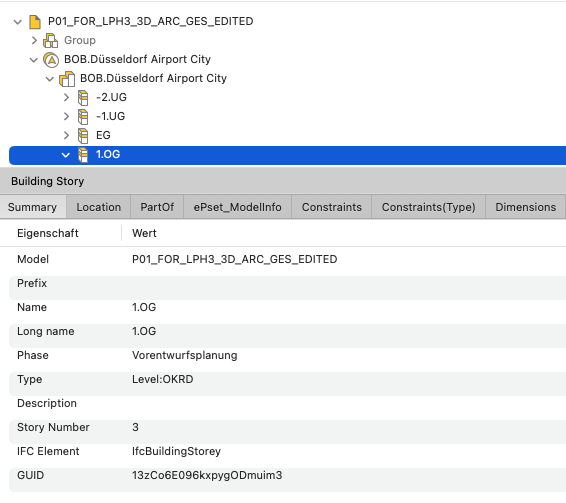
\includegraphics[width=0.6\textwidth]{doc/10/103_methods/bimcollab-zoom-example-selection.png}

	\caption[Beispielselektion eines Elementes in BIMcollab Zoom]{Auswahl eines IfcBuildingStorey-Elementes und dessen Psets und Properties in BIMcollab Zoom.}

	\label{fig:103_bimcollab-zoom-selection}
\end{figure}

Für komplexere Überprüfungen, besonders bei großen Mengen an Elementen, wurden Listen in BIMcollab Zoom eingesetzt.
Bei der Erstellung dieser Listen konnten verschiedene Suchkriterien ausgefüllt werden, um eine genaue Auswahl an Elementen aus dem digitalen Modell zu extrahieren.
Mit der Verwendung eines Pivot-Rasters, einer Unterkategorie der klassischen Liste, bestand zudem die Möglichkeit, arithmetische Funktionen auf den Properties der selektierten Elemente auszuführen.
In Abbildung \ref{fig:103_bimcollab-zoom-list} ist ein Pivot-Raster für die Berechnung der Fensterfläche in einem Modell dargestellt, das im Rahmen der Überprüfung eingesetzt wurde. \\

\begin{figure}[htb]
	\centering
		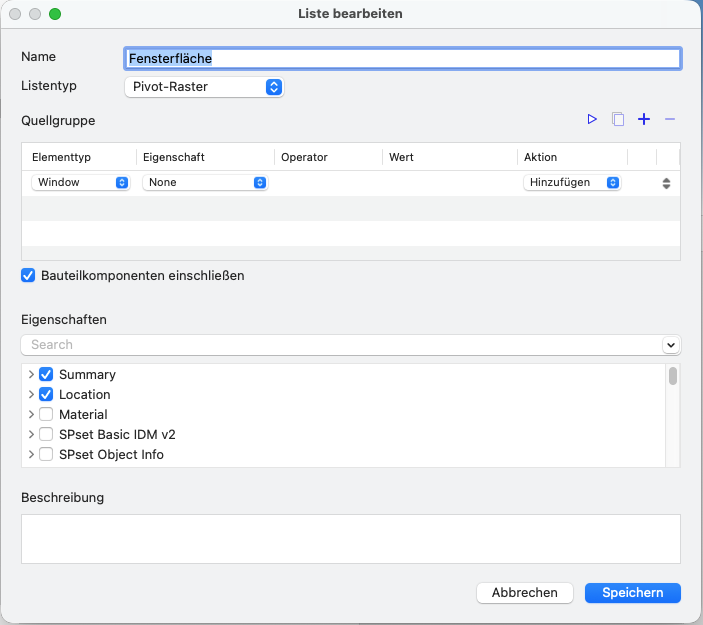
\includegraphics[width=0.6\textwidth]{doc/10/103_methods/bimcollab-zoom-example-list.png}

	\caption[Erstellung einer Liste in BIMcollab Zoom]{Erstellung eines Pivot-Rasters aller Fenster des Modells in BIMcollab Zoom.}

	\label{fig:103_bimcollab-zoom-list}
\end{figure}

Um die vom \gls{llm} verwendeten \gls{sql}-Abfragen zu überprüfen, wurde eine lokale Verwaltungssoftware für die manuelle Ausführung der generierten \gls{sql}-Abfragen verwendet.
Es handelte sich dabei um pgAdmin, eine für mehrere Betriebssysteme entwickelte Anwendung, die die Verwaltung verschiedener PostgreSQL-Datenbanken ermöglicht.
Neben der manuellen Ausführung von \gls{sql}-Abfragen wurde pgAdmin auch zur Analyse der Datenbankstruktur nach Migrationen oder zur Analyse einzelner Dateneinträge genutzt \cite{pgadmin2026features}.

\section{Aufbereitung der Daten}
\label{sec:datenaufbereitung}

Nach Abschluss der inhaltlichen Prüfung wurden die im Interviewverlauf entstandenen Daten in einem mehrstufigen Verfahren aufbereitet.
Zunächst erfolgte die strukturierte Erfassung aller Probanden einschließlich ihrer Gruppenzuordnung, um die späteren Auswertungen eindeutig den beiden Probanden-Gruppen zuordnen zu können.
Darauf aufbauend wurden die Kommunikationsverläufe in Form von Threads dokumentiert, wobei jeweils mehrere zusammenhängende Nachrichten einer konkreten Aufgabenstellung zugeordnet wurden.

Die zentrale Grundlage der weiteren Analyse bildete anschließend eine Tabelle mit sämtlichen \gls{llm}-Rückgaben.
Jeder Rückgabe wurde eine inhaltliche Kategorie zugewiesen; bei inkorrekten Ergebnissen wurde zusätzlich der vermutete Fehlergrund erfasst.
Auf diese Weise konnte neben der reinen Ergebnisdokumentation auch die qualitative Einordnung der Antworten nachvollziehbar festgehalten werden.
Die im Rahmen dieser Einordnung verwendeten Fehlerzustände sind in Tabelle \ref{tab:103_incorrect-output-errors} zusammengefasst.

\begin{table}[!htb]
    \centering
    \caption{Fehlerzustände bei inkorrekter \gls{llm}-Ausgabe}
    \label{tab:103_incorrect-output-errors}
    \begin{tabular}{C{4cm} L{9cm}}
        \hline
        \textbf{Name} & \textbf{Beschreibung}\\
        \hline

        Falsche \gls{ifc}-Entität genutzt & Bei der \gls{sql}-Abfrage wurde von dem \gls{llm} nach einer falschen \gls{ifc}-Entität gesucht. 
        Daraus ergab sich die Falschaussage, dass Daten nicht vorhanden wären oder es wurden unvollständige Daten angezeigt. \\

        Falsche Property/Pset genutzt & Im Rahmen der \gls{sql}-Abfrage wurde von dem \gls{llm} nach einer falschen Property oder einem falschen Pset gesucht. 
        Dies hat zur Folge, dass fälschlicherweise behauptet wurde, Daten seien nicht vorhanden, oder dass die angezeigten Daten unvollständig oder falsch waren. \\

        Falsches Werkzeug & Das \gls{llm} wählte bei der Bearbeitung ein falsches Werkzeug, sodass die ausgegebenen Daten teilweise oder vollständig falsch waren. \\

        \gls{sql}-Abfrage falsch aufgebaut & Die vom \gls{llm} erzeugte \gls{sql}-Abfrage wurde falsch aufgebaut. Dies können fehlende Filter, Gruppierungen oder falsche Aggregationen sein,
        was zu falschen Ergebnissen der Abfrage geführt hat. \\

        Sonstiger Fehler & Der Fehler hing nicht direkt mit dem \gls{llm} zusammen, sondern basierte auf Problemen mit der Datenbank, der eigentlichen Anwendung oder anderen vom \gls{llm} unabhängigen Parametern. \\

        \hline
    \end{tabular}
\end{table}

Ergänzend wurden die aufbereiteten Tabellen in einem gemeinsamen Datensatz zusammengeführt, sodass Rückgaben, Thread-Kontext und Probandengruppe gemeinsam ausgewertet werden konnten.
Im letzten Schritt wurde eine Aggregation der Daten durchgeführt, insbesondere auf Basis der kategorisierten \gls{llm}-Rückgaben und der dokumentierten Fehlerzustände.
Diese Verdichtung diente der Berechnung statistischer Kennzahlen und der Erstellung vergleichbarer Übersichten, die als Grundlage für die spätere Interpretation der Ergebnisse herangezogen wurden.